El dominio de la contratación pública electrónica comprende un conjunto de fases bien diferenciadas 
como ha quedado patente en el repaso realizado durante el Capítulo~\ref{capitulo:eprocurement}. De todas las 
fases identificadas y teniendo en cuenta las necesidades de interoperabilidad e integración, en general 
de comunicación, entre los distintos agentes implicados en este proceso administrativo, cabe destacar 
los procesos particulares de \textit{eAccess} y \textit{eNotification} en los cuales resulta 
especialmente relevante la publicación de información de forma estandarizada para impulsar 
la participación de cualquier tipo de organización creando un mercado competitivo de oportunidades 
a lo largo de toda una comunidad como es la Unión Europea. Si bien el caso de estudio de este documento 
se centra en los anuncios de licitación públicos a nivel europeo, el modelo propuesto es aplicable a 
cualquier otro entorno en los que las necesidades de compartir información sean un factor clave 
para el impulso de un sector de negocio.

Por otra parte, como se ha señalado en la Sección~\ref{10ders} existen una serie de problemas 
inherentes al proceso de contratación pública que no han sido abordados completamente o bien 
se han intensificado con el traspaso de la actividad a un entorno electrónico. En este sentido, 
la dispersión de la información, múltiples fuentes de datos, la heterogeneidad de los formatos tanto 
en publicación como en explotación y el multiling\"{u}ismo unido a la multiculturalidad, generan un entorno 
en el cual, evidentemente, el uso de semántica y la aplicación de los principios de \linkeddata pueden 
mejorar ostensiblemente su comportamiento, confiriendo el carácter transversal necesario a la información 
y datos que son utilizados y publicados bajo este proceso administrativo.

Los esfuerzos que se han llevado desde la gran mayoría de las instituciones públicas con intereses 
en impulsar la contratación pública por medios electrónicos ha generado la aparición de múltiples proyectos, 
plataformas, especificaciones, etc. que aunque si bien han atacado las necesidades de este entorno, también 
han generado un maremágnum de modelos, sub-procesos, pasos y etapas, etc. perjudicando en cierta medida 
las intenciones iniciales y absorbiendo gran parte del esfuerzo y del tiempo en la realización de 
acciones integradoras en vez de la generación de servicios de valor añadido para los agentes 
implicados.

De forma sintética esta introducción motiva el guía el proceso de aplicación del ciclo de vida 
de datos enlazados a los anuncios de licitación públicos.

\subsection{Proceso de Producción de \linkeddata de Anuncios de Licitación}
Atendiendo a la definición realizada en la Sección~\ref{sect:produccion}, este proceso 
implica aquellas tareas que a partir de un \dataset de entrada $\mathcal{G}$ y un conjunto 
de reglas de \textit{mapeo} $\mathcal{M}$ obtiene un \dataset \gls{RDF} $\mathcal{D}$ como resultado. Para la realización 
del proceso de producción y como quedará patente en las siguientes secciones se ha utilizado un programa 
Java desarrollado en particular para dar cobertura a esta transformación debido al tamaño y extensión 
de los datos disponibles, en total un millón de anuncios de licitación.

\subsubsection{Tarea $t_1$-Análisis del \dataset a transformar}\label{t1-ppn}
La casuística del proceso de contratación pública electrónica ha conllevado la realización 
de múltiples modelos de datos capaces de recoger y representar la información implicada 
en este proceso administrativo. De acuerdo a las especificaciones desarrollados en CODICE o en 
\gls{opXML} y según los modelos desarrollados en las ontologías propuestas por el proyecto LOTED 
y por la\textit{Charles University} de la República Checa, queda reflejado que la cobertura total 
de este proceso es verdaderamente complicada, por lo que es preferible la construcción 
de modelos de un tamaño sostenible y que dispongan de una gran capacidad de extensión 
e integración con otros ya existentes. Esta tendencia en el modelado de ontologías 
se ha considerado debido a que los intentos de realizar grandes especificaciones formales 
de distintos dominios no ha obtenido los beneficios deseados ya sea por su incapacidad para 
realmente representar todo el conocimiento o bien por el coste de realización de ciertos 
procesos automáticos como el razonamiento. Es por ello, que una buena práctica reside 
en la partición de conocimiento para así ofrecer modelos sencillos, representativos, flexibles 
e intrínsecamente extensibles.

En cuanto a las reglas de negocio o conocimiento que se encuentra en un modelo o especificación 
de la información de los datos de los anuncios de licitación cabe destacar los siguientes:
\begin{itemize}
 \item En un proceso de licitación se puede publicar un lote de anuncios de licitación 
de distinto tipo.
\item Un anuncio de licitación está identificado de forma única y se publica en al menos 
una fuente.
\item La publicación de un anuncio de licitación se realiza en al menos un idioma.
\item Un anuncio de licitación puede tener un anuncio previo, una adjudicación provisional o definitiva.
\item Un anuncio previo se identifica a través de un código y una fuente, además dispone de una fecha 
prevista de licitación, información sobre los lotes, información sobre el tipo de proceso (restringido, 
emergencia, central de contratación, etc.) para el cual se adjuntan una serie de documentos o pliegos.
\item El anuncio de licitación está compuesto por al menos un lote, dispone de la información 
de compra, es decir la adquisición que se realiza en el lote. De nuevo tiene asociado un proceso 
de licitación al cual se adjuntan una serie de documentos o pliegos.
\item La notificación provisional de adjudicación es relativa a un lote y en consecuencia a una 
adquisición de compra dentro de un determinado proceso para el cual existen documentos o pliegos. Evidentemente, 
consta de una serie de resoluciones entre las cuales se encuentra la provisional y la definitiva. Además, aparece 
la figura de las organizaciones implicadas.
\item La notificación definitiva de adjudicación consta de los mismos elementos que la anterior pero realizada 
de forma firme.
\item El proceso de contratación pública puede constar de un anuncio previo, un anuncio de licitación y las notificaciones 
provisional (opcional) y definitiva, para cada uno de ellos existe una serie de documentos asociados. Como metainformación 
se extrae: la descripción, fechas límites y eventos (localización, fecha inicio, fecha fin y persona de contacto).

\item Un lote dentro de anuncio de licitación tiene una adquisición de compra de un producto o servicio y una serie 
de resoluciones.
\item La adquisición está relacionada con un lote, sus notificaciones y anuncios, además de suministrar información 
sobre el tipo, título y descripción de compra, lista de códigos de adquisición, lista de items de adquisición (tipo y cantidad),
importe y localización.
\item La resolución de un lote tiene asociada una descripción, resultado y fecha además de datos de ofertas (items y cantidades) con 
un importe determinado en un moneda específica.
\item El importe de una adquisición tiene una cantidad total y otra sin impuestos, que se desglosan en cada tipo 
de índice de impuesto con una descripción asociada. Además, la cuantía se expresa en una moneda determinada.
\item La localización de cualquier anuncio, lote, etc. consta de una dirección postal, una localidad, un país y un idioma. El idioma 
puede estar asociado al país o a la región y desciendo hasta el grado de comunidad de autónoma (si nos referimos a España).
\item Una organización implicada en un proceso de licitación debe proveer información postal y una persona de contacto con 
cargo, teléfono, correo postal, nombre, etc.
\item Cualquier documento en todo el proceso de licitación tiene un título, una fecha y una descripción en un determinado 
idioma y está asociado a un pliego oficial.
\item Una fuente de publicación es aquella que se identifica por un código, un nombre, una descripción y una URL, además 
pertenece a una organización que realiza publicaciones en un determinado idioma.
\end{itemize}

El universo de discurso expuesto en la lista anterior guía el modelado posterior de la base de conocimiento 
y de los datos ya que debe cubrir las entidades identificadas para que toda la metainformación presente 
en los anuncios de licitación quede representada en las entidades del dominio. 

\subsubsection{Tarea $t_2$-Limpieza de datos}
Las fuentes de datos de anuncios de licitación son variadas y están disponibles en distintos formatos, en este 
trabajo y debido a la disponibilidad de datos de anuncios de licitación ya filtrados, facilitados por la 
empresa Euroalert.net, se ha decido utilizar este \dataset de entrada, en formato \gls{CSV}, en el cual la información ya ha sido 
recogida e integrada, evitando así la necesidad de recuperar información de distintas fuentes y de ejecutar 
tareas propias de la limpieza de datos. Aunque tratándose de fuentes públicas datos se pudiera pensar 
que la información oficial ya debería estar disponible de forma homogénea, la realidad es que la diversidad 
de formatos provoca un caos en el cual el esfuerzo para limpiar los datos consume gran parte del tiempo. No obstante, 
el sistema \gls{MOLDEAS} se ha diseñado mediante un conjunto de adaptadores de tal forma que la fuente de datos es independiente 
pudiendo generar representaciones semánticas para la mayoría de las fuentes de datos habituales a nivel nacional y 
europeo.

\subsubsection{Tarea $t_3$-Selección de Vocabularios}
Los vocabularios seleccionados para modelar los anuncios de licitación teniendo en cuenta el análisis 
 realizado en la tarea $t_1$ se presentan en la Tabla~\ref{table:ppn-select-vocabs}. En general, se trata de vocabularios 
 que atienden a los siguientes criterios:
% 
\begin{enumerate}
  \item Formalización de una estructura taxonómica, como RDFS, \gls{SKOS} u \gls{OWL}.
  \item Realización de \textit{mapeos} entre conceptos, como SKOS y OWL.
  \item Representación de tipos de datos, como \gls{XML Schema}.
  \item Gestión de información multiling\"{u}e, como \gls{SKOS-XL} y RDFS.
  \item Adición de metadatos y provenance, como Dublin Core Terms, \gls{voID} y Provenance Ontology.
  \item Representación del tiempo e intervalos, como Time Ontology del \gls{W3C}.
 \end{enumerate}


\begin{longtable}[c]{|l|p{4cm}|p{4cm}|p{4cm}|} 
\hline
\textbf{Prefijo} &  \textbf{Vocabulario} &  \textbf{Fuente} & \textbf{Uso} \\\hline
\endhead
 c4n & \url{http://vocab.deri.ie/c4n#}& Michael Hausenblas & Especificación de llamadas para participar en eventos. \\ \hline  
 dbpedia & \url{http://dbpedia.org/ontology/}&  Comunidad \linkeddata. & Reutilización de definiciones. \\ \hline 
 dc11 & \url{http://purl.org/dc/elements/1.1/}&  Dublin Core Metadata Initiative & Creación de metadatos para los documentos. \\ \hline  
 dct & \url{http://dublincore.org/documents/dcmi-terms/}&  $\equiv$ & $\equiv$ \\ \hline  
 dol & \url{http://www.loa-cnr.it/ontologies/DOLCE-Lite.owl#}&  \textit{WonderWeb Foundational Ontologies Library} & Ontología estructural. \\ \hline
 edns  &  \url{http://www.loa-cnr.it/ontologies/ExtendedDnS.owl#}& $\equiv$ & $\equiv$ \\ \hline
 mod  &  \url{http://www.loa-cnr.it/ontologies/ModalDescriptions.owl#}& $\equiv$ & $\equiv$ \\ \hline
 mads  &  \url{http://www.loc.gov/mads/rdf/v1#>}& $\equiv$ & $\equiv$ \\ \hline
 foaf & \url{http://xmlns.com/foaf/0.1/} &Comunidad de Web Semántica.& Especificación de relaciones entre personas. \\ \hline 
 gr & \url{http://purl.org/goodrelations/v1#} & Martin Heep & Reutilización de definiciones para describir productos y servicios.\\\hline 
 geo & \url{http://www.w3.org/2003/01/geo/wgs84_pos#} & W3C & Reutilización de elementos geográficos.\\\hline 
 lgd & \url{http://linkedgeodata.org/ontology/} & \textit{Linked Geodata Initiative} & $\equiv$\\\hline 
 org  & \url{http://www.w3.org/ns/org#} & Epimorphics Ltd. & Descripción de organizaciones. \\ \hline
 owl  & \url{http://www.w3.org/2002/07/owl#} & W3C & Realización de definiciones en el dominio. \\\hline
 po & \url{http://www.productontology.org/} & Martin Heep & Reutilización de datos provenientes de Productontology.\\\hline 
 prov  & \url{http://purl.org/twc/ontology/w3c/prov#} & W3C & Especificación de metadatos de procedencia. \\\hline 
 payment  & \url{http://reference.data.gov.uk/def/payment#} & Gobierno de Reino Unido & Especificación de pagos. \\\hline
 pscs  & \url{http://purl.org/weso/pscs/ontology/} & Parte del estudio de esta tesis. &Ontología para las definiciones de las PSCs. \\\hline
 nuts  & \url{http://nuts.psi.enakting.org/def/} & Universidad de Southampton & Especificación de las regiones europeas. \\\hline
 qb & \url{http://purl.org/linked-data/cube#} & Comunidad \linkeddata & Especificación de datos estadísticos. \\ \hline
 skos & \url{http://www.w3.org/2004/02/skos/core#} & W3C & Especificación de taxonomías. \\ \hline
 skosxl & \url{http://www.w3.org/2008/05/skos-xl#>} & W3C & Representación de información ling\"uística. \\ \hline
 rdf & \url{http://www.w3.org/1999/02/22-rdf-syntax-ns#} & W3C & Descripción de recursos. \\ \hline
 rdfs & \url{http://www.w3.org/2000/01/rdf-schema#} & W3C & Descripción de recursos con relaciones lógicas. \\ \hline 
 time & \url{http://www.w3.org/2006/time#} & W3C & Especificación de intervalos de tiempo.\\\hline 
 time-entry & \url{http://www.w3.org/2006/time-entry#} & W3C & $\equiv$\\\hline  
 intervals & \url{http://reference.data.gov.uk/def/intervals/} & Gobierno de Reino Unido & $\equiv$ \\\hline 
 vann & \url{http://purl.org/vocab/vann/} & Ian Davis & Anotación de los vocabularios. \\\hline
 vcard & \url{http://www.w3.org/2006/vcard/ns#} & W3C & Representación de información de contacto. \\\hline
 void & \url{http://rdfs.org/ns/void#} & Deri y W3C & Descripción de metadatos de un \dataset. \\\hline
 xml & \url{http://www.w3.org/XML/1998/namespace} & W3C & Reutilización de definiciones. \\\hline
 xsd & \url{http://www.w3.org/2001/XMLSchema#} & W3C & Especificaciónd de tipos de datos. \\\hline
\hline
\caption{Selección de Vocabularios para los Anuncios de Licitación.}\label{table:ppn-select-vocabs}\\    
\end{longtable}
% 
\subsubsection{Tarea $t_4$-Selección de otros \datasets RDF}
En este caso el principal \dataset RDF a reutilizar es relativo a la información geográfica 
de países europeos denominado NUTS y cuyo uso se detalla en la Sección~\ref{sect:rdf-orgs}.

\subsubsection{Tarea $t_5$-Modelado de datos en RDF}
El resultado de esta tarea debe ser una ontología de dominio $\mathcal{O}$ que modele la información 
de los anuncios de licitación, $r_{ppn}$, pertenecientes a un \dataset RDF $\mathcal{D}$. Por lo tanto, se debe 
suministrar una ontología $\mathcal{O}$ de acuerdo al análisis realizado en la Sección~\ref{t1-ppn}, facilitando 
así la descripción formal de los datos de los recursos \gls{RDF}:
% 
 \begin{itemize}
  \item $\mathcal{C} = \{$\textit{Contract, Notice, Agreement, Document,...,AwardCriteria}$\}$
  \item $\mathcal{R} = \{$\textit{rdf:type, dc:identifier, dc:subject, dc:date...foaf:topic, ref-cpv, ref-nuts, rdfs:label}$\}$
  \item $\mathcal{I} = \{ r_{ppn} \}$
  \item $\mathcal{A} = \{\}$
 \end{itemize}
%  
 Como segundo paso se diseñan las propiedades que deben tener los recursos, teniendo en cuenta su ulterior aplicación ver 
Tabla~\ref{table:ppn-rdf-model},  pertenecientes a ese \dataset y que son comunes para todas los anuncios de licitación.
% 
\begin{longtable}[c]{|p{5cm}|p{4.5cm}|p{5cm}|} 
\hline
  \textbf{Propiedad} &  \textbf{Descripción} & \textbf{Ejemplo} \\\hline
  \texttt{rdf:type} & Especificación del tipo de un recurso del \dataset RDF & a \texttt{Contract}, \texttt{Notice} \\ \hline
  \texttt{dc:identifier} & Identificador utilizado en la URI del recurso &  \texttt{dc:identifier} "201898"$\textasciicircum\textasciicircum$xsd:string \\ \hline
  \texttt{dc:subject} & Identificador original proveniente de la fuente de datos &  \texttt{dc:subject} "201898"$\textasciicircum\textasciicircum$xsd:string \\ \hline
  \texttt{dc:date} & Fecha de publicación del recurso &  \texttt{dc:date} "2008"$\textasciicircum\textasciicircum$xsd:date \\ \hline
  \texttt{dc:publisher} & Entidad emisora &  \texttt{dc:publisher} <http://ec.europa.eu/> \\ \hline
  \texttt{foaf:topic} & Tipo de licitación (códigos CPV) &  \texttt{foaf:topic} cpv2008:60400000 \\ \hline
  \texttt{ref-cpv} & $\equiv$ &  \texttt{ref-cpv} cpv2008:60400000 \\ \hline
  \texttt{ref-nuts} & Localización del anuncio de licitación &  \texttt{ref-nuts} nuts:FR \\ \hline
  \texttt{rdfs:label} & Etiqueta o título del anuncio de licitación &  "Anuncio de licitación"$\textasciicircum\textasciicircum$xsd:string \\ \hline
  \texttt{dc:title} & $\equiv$  &  "Anuncio de licitación"$\textasciicircum\textasciicircum$xsd:string \\ \hline
  \texttt{rdfs:description} & Descripción del anuncio de licitación &  "Descripción del Anuncio de licitación"$\textasciicircum\textasciicircum$xsd:string \\ \hline
  \multicolumn{3}{|c|}{\ldots} \\ \hline
\endhead
\hline
\caption{Diseño de propiedades para de los Anuncios de Licitación.}\label{table:ppn-rdf-model}\\    
\end{longtable}
% 
Una vez establecido el conjunto de propiedades de cada recurso \gls{RDF} representando un 
anuncio de licitación, es necesario definir el conjunto de grafos en los cuales se encuadrarán 
los recursos, es decir, el \dataset RDF $\mathcal{D}$. Para ello, 
en la Tabla~\ref{table:ppn-dataset} se indican las tuplas $(\mathcal{G}_k, I_k)$ correspondientes a cada uno 
de los grafos $\mathcal{G}_k$ identificados a través de la URI $I_k$.
% 
\begin{longtable}[c]{|p{3cm}|p{9cm}|} 
\hline
  \textbf{$\mathcal{G}_k$} &  \textbf{$I_k$}  \\\hline
\endhead
 \textbf{$\mathcal{G}$}   & \url{http://purl.org/weso/ppn} \\ \hline
 \textbf{$\mathcal{G}_1$} & \url{http://purl.org/weso/ppn/2008} \\ \hline
 \textbf{$\mathcal{G}_2$} & \url{http://purl.org/weso/ppn/2009} \\ \hline
 \textbf{$\mathcal{G}_3$} & \url{http://purl.org/weso/ppn/2010} \\ \hline
 \textbf{$\mathcal{G}_4$} & \url{http://purl.org/weso/ppn/2011} \\ \hline
 \textbf{$\mathcal{G}_{5}$} & \url{http://purl.org/weso/ppn/ontology} \\ \hline 
\hline
\caption{\textit{Dataset} RDF $\mathcal{D}$ para Anuncios de Licitación.}\label{table:ppn-dataset}\\    
\end{longtable}
% 
% 
\subsubsection{Tarea $t_6$-Diseño de un Esquema de URIs}
Esta tarea tiene como objetivo establecer la forma y estructura de las URIs para las definiciones 
realizadas en la ontología $\mathcal{O}$ como para todos los recursos presentes en el \dataset RDF $\mathcal{D}$ que 
se genera a partir de la transformación de los datos a \gls{RDF}. Es una de las actividades clave ya que guiará 
tanto el método final de transformación como el proceso posterior de publicación. En la Tabla~\ref{table:ppn-uris} se 
hace la descripción de la estructura de \gls{URI}s que se utilizarán en la generación de los anuncios de licitación. Se ha optado 
por un diseño en el cual las URIs refieren a la información más útil y única, abordando la descripción pormenorizada 
de cada uno de los recursos a través de las propiedades, evitando así la generación de URIs excesivamente extensas con 
mucha metainformación.
% 
\begin{longtable}[c]{|p{5cm}|p{4.5cm}|p{5cm}|} 
  \textbf{URI} &  \textbf{Descripción} & \textbf{Ejemplo} \\\hline
\endhead
\url{http://purl.org/weso/ppn/} & URI base: <base\_uri> & NA \\ \hline
\url{<base_uri>/ontology} & Definiciones comunes a todos los anuncios de licitación & \url{<base_uri>/ontology/Contract} \\ \hline
\url{<base_uri>/resource/ds} & Descripción del catálogo de los anuncios de licitación & \url{<base_uri>/resource/ds} \\ \hline
\url{<base_uri>/ppn/{year}} & Espacio de nombres para una determinada PSC & \url{<base_uri>/ppn/2008} \\ \hline
\url{<base_uri>/resource/ppn/{year}/{id}} & URI para un recurso representando un anuncio de licitación & \url{<base_uri>/ppn/2008/201898} \\ \hline
\hline
\caption{Diseño de URIs para los Anuncios de Licitación.}\label{table:ppn-uris}\\    
\end{longtable}

\subsubsection{Tarea $t_7$-Diseño Plantilla Objetivo del Recurso RDF}
El objetivo de esta tarea es establecer una plantilla de cada uno de los recursos RDF que están 
presentes en el \dataset RDF $\mathcal{D}$ para que sirvan como guía en los siguientes momentos: 1) en la ejecución propiamente dicha 
de la transformación de los datos originales a \gls{RDF} y 2) en la validación de los recursos RDF generados. De esta manera, 
tratándose de \datasets con una gran cantidad de recursos se puede fácilmente identificar recursos que no sean 
compatibles con este esquema favoreciendo la depuración de los recursos generados. Adicionalmente, un esquema de 
recurso sirve como documentación extra para el proceso de consumo. 
%
De acuerdo al recurso plantilla, ver Figura~\ref{fig:ppn-template}, y a las definiciones realizadas en la ontología que modela estos datos 
es posible realizar una validación en cuanto a los tipos de datos, cardinalidad de las relaciones, tipo de objetos, etc., que 
resulta de sumo interés para asegurar la calidad de los datos producidos.
 
 \begin{figure}[!htp]
 \begin{lstlisting} 
<<base_uri>/resource/ppn/{year}/{id}>
      a       Notice;
     (rdfs:label ""@lang ;)+
     (rdfs:description ""@lang ;)+
     dc:identifier ""^^xsd:string ;
     dc:subject ""^^xsd:string ;
     dc:title ""^^xsd:string ;
     dc:date ""^^xsd:date ;
     (foaf:topic <uri>;)*
     (ref-cpv <uri>;)*
     (ref-nuts <uri>;)*
      ...
      .	
\end{lstlisting}
	\caption{Plantilla Objetivo de un Recurso de los Anuncios de Licitación.}
	\label{fig:ppn-template}
\end{figure}
% 
% 
% 
\subsubsection{Tarea $t_8$-Enriquecimiento de los datos en RDF}\label{t8-pscs}
En el caso de los anuncios de licitación la tarea de enriquecimiento se ha realizado 
en las propias clasificaciones de productos y en las organizaciones (países y localización). Directamente, 
se ha optado por evitar el enriquecimiento de los anuncios de licitación manteniendo así la información 
original de la forma más clara y sencilla posible. Evidentemente, la Tarea $t_{10}$ sobre ``Reconciliación de Entidades'' 
se ha delegado ya que además de proveer enlaces a los documentos oficiales en las fuentes no existen fuentes 
de datos semánticas en las cuales se disponga información extra sobre una determinada licitación.
% 
\subsubsection{Tarea $t_9$-Transformación de los datos a RDF }
Una vez realizadas las tareas anteriores se está en disposición de realizar la transformación 
de los datos de entrada a \gls{RDF}. En esta tarea el punto clave de decisión reside en seleccionar o bien 
una herramienta ya disponible o bien implementar un programa que ejecute las reglas de transformación 
tomando como entrada los datos de las clasificaciones. En esta caso, se ha optado por la implementación 
de un proceso Java particular debido a la casuística y el tamaño del \dataset de entrada.
% 
\subsubsection{Tarea $t_{16}$-Añadir metainformación a los recursos RDF}\label{t16-ppn}
En relación a la metainformación en los anuncios de licitación y teniendo en cuenta 
la interpretación posible realizada en la Sección~\ref{t16-metodos} se ha optado 
por un enfoque mixto en el cual se provee la descripción de los propios 
\datasets \gls{RDF}, ver Figuras~\ref{fig:ppn-ls} y~\ref{fig:ppn-ds-2008} además de indicar en 
cada recurso su información particular de procedencia. Es relevante destacar 
la definición de la licencia de los datos con el objetivo de facilitar 
su posterior reutilización, en este caso se ha optado por una licencia de ``Open Data'' basada en las 
directrices fijadas en la guía provista en~\cite{od-license}.
% 
\begin{figure}[!htp]
\begin{lstlisting} 
<http://purl.org/weso/ppn/data/resource/ds?output=ttl>
      rdfs:label "RDF description of Public Procurement Notices" ;
      foaf:primaryTopic <http://purl.org/weso/ppn/resource/ds> .

<http://purl.org/weso/ppn/resource/ds>
      a    <http://rdfs.org/ns/void#Linkset> ;
      rdfs:label "Public Procurement Notices"@en ;
      dcterms:author 
            <http://www.di.uniovi.es/~labra/labraFoaf.rdf#me> , 
	    <http://www.josemalvarez.es/foaf.rdf#me> ;
      dcterms:contributor
            <http://purl.org/weso/pscs/resource/10ders> ,
	    <http://rdfohloh.wikier.org/project/moldeas/rdf> ;
      dcterms:description 
            "Some Public Procurement Notices available in RDF" ;
      dcterms:license
            <http://opendatacommons.org/licenses/by/1.0/> ;
      dcterms:modified
            "2011-11-10"^^<http://www.w3.org/2001/XMLSchema#date> ;
      dcterms:publisher
            <http://www.josemalvarez.es/foaf.rdf#me> ;
       dcterms:title
            "Public Procurement Notices" ;
      void:target
            <http://purl.org/weso/ppn/2008/resource/ds> , 
            <http://purl.org/weso/ppn/2009/resource/ds> , 
            <http://purl.org/weso/ppn/2010/resource/ds> , 
            <http://purl.org/weso/ppn/2011/resource/ds> ;
      foaf:homepage <http://purl.org/weso> .	
\end{lstlisting}
	\caption{Descripción del \textit{Linkset} de los Anuncios de Licitación.}
	\label{fig:ppn-ls}
\end{figure}


\begin{figure}[!htp]
\begin{lstlisting} 
<http://purl.org/weso/pscs/ppn/2008/resource/ds>
      a       void:Dataset , skos:ConceptScheme ;
      rdfs:label "Public Procurement Notices 2008"@en ;
      dcterms:author 
            <http://www.di.uniovi.es/~labra/labraFoaf.rdf#me> , 
	    <http://www.josemalvarez.es/foaf.rdf#me> ;
      dcterms:contributor
            <http://purl.org/weso/pscs/resource/10ders> ,
	    <http://rdfohloh.wikier.org/project/moldeas/rdf> ;
      dcterms:description "Common Procurement Vocabulary" ;
      dcterms:license <http://opendatacommons.org/licenses/by/1.0/> ;
      dcterms:modified "2011-06-06"^^xsd:date ;
      dcterms:publisher <http://www.josemalvarez.es/foaf.rdf#me> ;
      dcterms:source 
	<http://europa.eu/legislation_summaries/internal_market/businesses/public_procurement/l22008_en.htm> ;
      dcterms:title "PPN 2008" ;
      void:dataDump <http://purl.org/weso/pscs/ppn/2008/ppn-2008.ttl> ;
      void:exampleResource
        <http://purl.org/weso/ppn/2008/resource/18000000> , 
	<http://purl.org/weso/ppn/2008/resource/45000000> , 
	<http://purl.org/weso/ppn/2008/resource/33000000> ;
      void:uriRegexPattern
        "http://purl.org/weso/ppn/2008/resource/.+" ;
      void:vocabulary skosxl: , skos: , rdfs: ;
      foaf:homepage <http://purl.org/weso> .
\end{lstlisting}
	\caption{Descripción del \dataset de Anuncios de Licitación 2008.}
	\label{fig:ppn-ds-2008}
\end{figure}
 
\cleardoublepage
% 
\subsubsection{Resultado Final y Ejemplos}
El resultado final del proceso de producción de \linkeddata tras el análisis y ejecución 
de las tareas identificadas y del método de producción seleccionado genera como resultado un conjunto de 
datos en \gls{RDF} mediante datos enlazados en los cuales se pueden extraer las siguientes 
estadísticas de producción de datos, ver Tabla~\ref{table:ppn-ejemplos}, consultas, ver Figura~\ref{fig:ppng-sparql-query} y un 
ejemplo conteniendo la información básica de los recursos generados, ver Figura~\ref{fig:ppn-example-2008}. 

\begin{Frame}
 \textit{``Dame 100 anuncios de licitación en el campo de maquinaría industrial que se han solicitado 
en Francia e Inglaterra durante el año 2008 y 2009''}
\end{Frame}
% 
% 
\begin{longtable}[c]{|p{2.5cm}|p{2.5cm}|p{1.8cm}|p{1.8cm}|} 
\hline
  \textbf{Anuncios de Licitación} & \textbf{Nº de Elementos}  &  \textbf{Ejemplo} &  \textbf{Tripletas}  \\\hline
\endhead
PPN 2008 & $112843$  & Figura~\ref{fig:ppn-example-2008}   &  $677058$  \\ \hline
PPN 2009 & $399766$ &  $\equiv$   & $2398601$   \\ \hline
PPN 2009  & $431813$& $\equiv$     & $2590880$  \\ \hline
PPN 2011 & $67044$&  $\equiv$    & $402264$   \\ \hline
\multicolumn{4}{|c|}{\textbf{Catálogo de Anuncios de Licitación} (total)} \\ \hline
PPNs & $1011466$ &  N/A & $6068803$   \\ \hline
\hline
\caption{Estadísticas y Ejemplos de los Anuncios de Licitación.}\label{table:ppn-ejemplos}\\    
\end{longtable}
% 
\begin{figure}[!htp]
\begin{lstlisting} 
SELECT DISTINCT * WHERE{
  ?ppn rdf:type :Notice.
  ?ppn ref-nuts ?nutsCode.
  FILTER(?nutsCode = <http://nuts.psi.enakting.org/id/UK> or 
    ?nutsCode = <http://nuts.psi.enakting.org/id/FR> ) .
  ?ppn ref-cpv ?cpvCode. 
  FILTER(?cpvCode = cpv2008:42000000 ) .
  ?ppn dc:identifier ?id.
  ?ppn dc:date ?date . 
  FILTER ( (xsd:long(?date) >=  xsd:long(2008)) 
    && (xsd:long(?date) <=  xsd:long(2009)) )
} LIMIT 100
\end{lstlisting}
	\caption{Ejemplo de consulta en SPARQL sobre los Anuncios de Licitación.}
	\label{fig:ppng-sparql-query}
\end{figure}
% 
% 
% 
\begin{figure}[!htp]
	\lstinputlisting{examples/e-proc/ppn-2008.ttl}
	\caption{Ejemplo final básico de un Anuncio de Licitación en RDF.}
	\label{fig:ppn-example-2008}
\end{figure}

%
\subsubsection{Método de Producción de \linkeddata de Anuncios de Licitación}
De acuerdo al análisis y diseño de datos enlazados realizado para los anuncios de licitación
a lo largo de las anteriores anteriores y la tabla de decisión~\ref{tabla:produccion}, el método semántico seleccionado 
para realizar la producción de datos enlazados es el $SPM_1$-``Transformación de datos a RDF'', ver Sección~\ref{spm-1}, en el 
se transforman un conjunto de datos de entrada $\mathcal{G}$ a un \dataset RDF $\mathcal{D}$. Según la definición de método 
semántico de producción, realizada en la Sección~\ref{method-prod-def}, y el estudio de los anuncios de licitación se pueden 
establecer los siguientes conjuntos:
\begin{itemize}
 \item $\mathcal{G}$ es el \dataset de entrada, conjunto de tuplas, conteniendo los datos de cada uno de los anuncios de licitación.
 \item $\mathcal{M}$ es el conjunto de \textit{mapeos}, ver Tabla~\ref{tabla:produccion-ppn}, extraídos según el análisis y diseño realizado en las secciones anteriores. Estos 
\textit{mapeos} son directamente expresables en la herramienta de transformación y toman como parámetros el valor de una de las tuplas de entrada (posición $X$) y la propiedad a generar.
 \item \textit{Dataset} \gls{RDF} $\mathcal{D}$ es el \dataset resultado, igualmente, siguiendo el análisis y diseño realizado en las secciones anteriores y tras la ejecución 
de la tarea propia de transformación de datos.
\end{itemize}
% 

\begin{longtable}[c]{|p{2cm}|p{8cm}|p{4cm}|} 
\hline
  \textbf{$\mathcal{M}$} &  \textbf{Propiedad} & \textbf{Valor} \\\hline
\endhead
 $m_1$ & \texttt{rdf:type} & URI \\ \hline
 $m_2$ & \texttt{dc:identifier} & \texttt{xsd:string} \\ \hline
 $m_3$ & \texttt{dc:subject} & \texttt{xsd:string} \\ \hline
 $m_4$ & \texttt{dc:date} & \texttt{xsd:string}   \\ \hline
 $m_5$ & \texttt{dc:title} & \texttt{xsd:string}   \\ \hline
 $m_6$ & \texttt{dc:publisher} &  URI  \\ \hline
 $m_7$ & \texttt{ref-cpv} & URI \\ \hline
 $m_8$ & \texttt{ref-nuts} & URI  \\ \hline
 $m_{9}$ & \texttt{foaf:topic} & URI \\ \hline  
 $m_{10}$ & \texttt{rdfs:label} & \texttt{xsd:string@lang} \\ \hline
 $m_{11}$ & \texttt{rdfs:description} & \texttt{xsd:string@lang} \\ \hline    
  \multicolumn{3}{|c|}{\ldots} \\ \hline  
\hline
\caption{Conjunto de \textit{mapeos} $\mathcal{M}$ para los Anuncios de Licitación.}\label{tabla:produccion-ppn}\\    
\end{longtable}
% 
\subsection{Proceso de Publicación de \linkeddata de Anuncios de Licitación}\label{sect:proceso-publicacion-ld}
Según la definición realizada en la Sección~\ref{sect:publicacion}, este proceso conlleva
todas las tareas que implican la publicación de un \dataset RDF $\mathcal{D}$ a través de un conjunto 
de características $\mathcal{P}$ para la obtención de un \dataset RDF $\mathcal{D}_{pub}$, método semántico 
de publicación. El método seleccionado para la publicación de datos es una conjunción 
de los detallados en las Secciones~\ref{spm-1-pub} (Fichero estático \gls{RDF}),~\ref{spm-3-pub} (\textit{Endpoint} de SPARQL) y~\ref{linkeddata-frontend} 
(\linkeddata \textit{Frontend}) con el objetivo de dar cobertura a las necesidades de la mayor parte de los potenciales clientes. De esta forma, 
se suministra un entorno en el cual se pueden: 1) descargar todos los datos de una única consulta y un sólo formato de datos; 2) realizar consultas personalizadas 
con distintos formatos de salida a través del protocolo y lenguaje propuesto en \gls{SPARQL} y 3) navegar a través de los datos mediante un interfaz con provisión 
para la negociación de contenido. 
% 
% Debido al ingente conjunto de características del conjunto $\mathcal{P}$ para la publicación a través de la web, incluyendo las propias de HTTP, en la Tabla~\ref{table:pscs-publish} 
% se indican aquellas más importantes de acuerdo a los métodos de publicación seleccionados.
% 
% \begin{longtable}[c]{|p{2cm}|p{8cm}|p{4cm}|} 
% \hline
%   \textbf{$\mathcal{P}$} &  \textbf{Característica} & \textbf{Valor} \\\hline
% \endhead
%  $\mathcal{p}_1$ &  HTTP  & FIXME \\ \hline
% 
% \hline
% \caption{Conjunto de características $\mathcal{P}$ de publicación para las Clasificaciones Estándar de Productos.}\label{table:pscs-publish}\\    
% \end{longtable}
% 
% 
\subsubsection{Tarea $t_{14}$-Infraestructura para \linkeddata}\label{infraestructura-comun}
El objetivo de esta tarea es el diseño de la infraestructura necesaria para albergar los datos enlazados, permitiendo 
así el acceso a los mismos y su consiguiente reutilización siguiendo los métodos de publicación seleccionados. Dependiendo de los servicios a ofrecer se deberán contemplar 
distintos componentes software aunque un ejemplo característico del posible diagrama despliegue será el que se puede 
observar en la Figura~\ref{fig:infra-ld} y que se utilizará como representativo para el contexto de los anuncios de licitación, 
incluyendo las clasificaciones de productos y las organizaciones. 

\begin{figure}[!htp]
\centering
	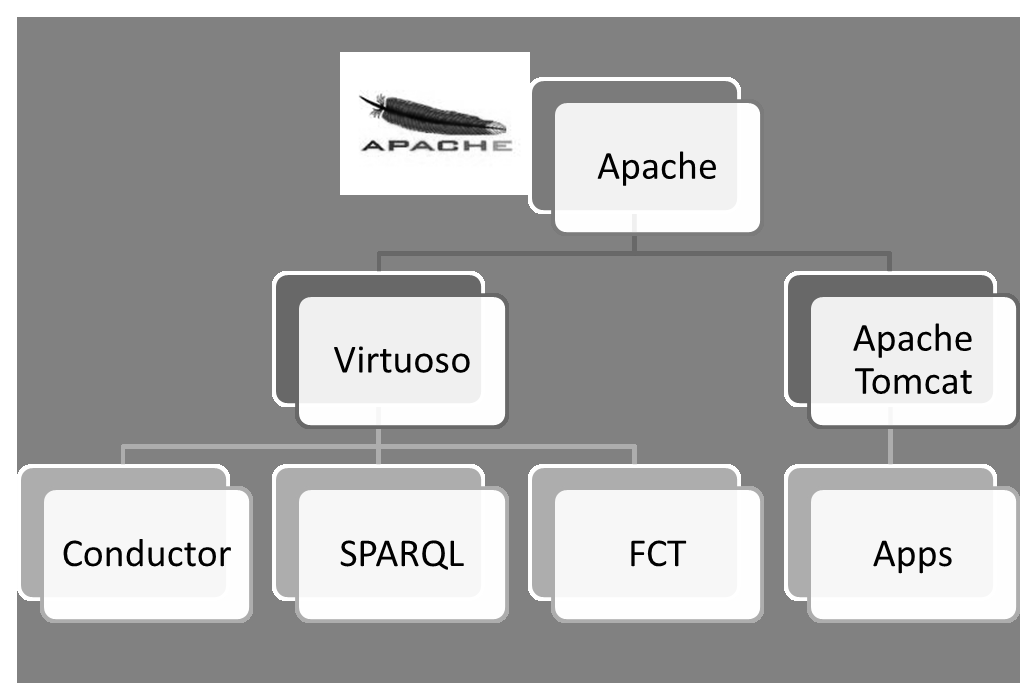
\includegraphics[width=10cm]{images/phd/infra-ld}
	\caption{Infraestructura Objetivo para \linkeddata.}
	\label{fig:infra-ld}
\end{figure}

Cada uno de estos componentes cumple una función específica que se detalla a continuación:
\begin{description}
 \item [Servidor web.] Teniendo presentes dos de los grandes objetivos de la publicación de datos enlazados como son el uso 
de HTTP URIs y que éstas sean en el mayor grado posible \textit{cool uris}, la presencia de un servidor web se justifica como punto 
de entrada a la consulta de los datos enlazados evitando la presencia de números de puerto, etc. y suministrando un acceso 
homogéneo a los datos. Para el cumplimiento de estos objetivos se ha seleccionado el servidor web Apache2. Por otra parte, con una configuración 
del servidor se da soporte al método de publicación basado en un ``\textit{Fichero estático RDF}''.
\item [Servidor de aplicaciones.] Este componente es el encargado de albergar las aplicaciones que proporcionan servicios de valor añadido 
de acceso a los datos desde diferentes puntos de vista. También se puede desplegar un contenedor de servlets que en muchos casos es suficiente. En este caso, 
seleccionando Pubby como elemento de software para dar soporte al método de publicación mediante un ``\linkeddata \textit{Frontend}''.
\item [Repositorio RDF.] Con el objetivo de albergar los datos transformados en RDF, es decir el \dataset RDF $\mathcal{D}$ es necesario el despliegue 
de un servidor RDF, para esta tarea existen diferentes opciones~\cite{5638466} pero Virtuoso de OpenLink se considera una buena opción por su amplia aceptación, 
capacidad de extensión y soporte a las especificaciones.
\item [\textit{Endpoint} de \gls{SPARQL}.] Del mismo modo que los datos transformados se han de almacenar también es conveniente proveer un interfaz de acceso 
a los mismos mediante el protocolo y lenguaje de consulta SPARQL. Igualmente existen diferentes opciones, sin embargo como parte de Virtuoso existe un módulo 
que se instala y está disponible automáticamente con el despliegue inicial del repositorio. El comportamiento de este componente se asemeja también a 
un servicio web \gls{REST} con peticiones GET facilitando de forma parcial otro método de publicación como el señalado en la Sección~\ref{servicio-web-produccion}.
\end{description}
% 
\subsubsection{Tarea $t_{15}$-Acceso y formato en datos RDF}\label{t15-comun}
Las necesidades de las aplicaciones para el posible consumo de datos varían ostensiblemente 
dependiendo de su objetivo. En el caso objeto de estudio de este documento y con la infraestructura 
indicada en la anterior sección se suministra soporte a los siguientes formatos de datos:

\begin{longtable}[c]{|p{4cm}|p{4cm}|p{4cm}|} 
\hline
  \textbf{Acceso} &  \textbf{Formato} &  \textbf{Provisto por}  \\\hline
\endhead
 Petición GET    & N3/Turtle    & Apache2 \\ \hline
 Consulta SPARQL & \textit{Spreadsheet}  & \textit{Endpoint} de SPARQL  \\ \hline
 $\equiv$        & XML 		& $\equiv$ \\ \hline
 $\equiv$        & JSON 	& $\equiv$ \\ \hline
 $\equiv$        & Javascript 	& $\equiv$  \\ \hline 
 Consulta SPARQL y petición GET      & N3/Turtle 	& \textit{Endpoint} de SPARQL y \linkeddata \textit{Frontend} \\ \hline
 $\equiv$        & RDF/XML 	& $\equiv$ \\ \hline
 $\equiv$        & NTriples 	& $\equiv$  \\ \hline
 $\equiv$        & HTML 	& $\equiv$  \\ \hline
 \hline
\caption{Acceso y Formato de datos de los Anuncios de Licitación.}\label{table:pscs-acceso}\\    
\end{longtable}

\subsection{Proceso de Consumo de Anuncios de Licitación}
El proceso de consumo de datos enlazados, según la definición realizada en la Sección~\ref{sect:proceso-consumo}, consiste en 
la reutilización de los datos enlazados para ser aplicados en la construcción de una nueva aplicación o servicio de valor 
añadido. En general, la reutilización más sencilla consiste en la representación gráfica de los recursos o la simple 
consulta con selección de formato de datos de acuerdo a las características de publicación utilizadas. En el caso 
que nos ocupa y teniendo en cuenta el objetivo de realización de un prototipo experimental de extracción de anuncios 
de licitación como demostrador del consumo de datos enlazados se ha escogido el método semántico de consumo $SCM_2$-``\textit{Mapeo} a Lenguaje de Programación'', 
cuya descripción está disponible en la Sección~\ref{scm2-consumo}, y orientado a obtener una representación de los recursos RDF en un 
lenguaje de programación (en este caso Java) como objetos de negocio. De acuerdo a este objetivo y la definición del propio método 
es necesario definir:
\begin{itemize}
 \item El \dataset RDF $\mathcal{D}_{pub}$, es el conjunto de datos disponible tras aplicar el método de publicación.
 \item El conjunto $\mathcal{M}^1$, ver Tabla~\ref{table:ppn-consumo}, indica como transformar el \dataset anterior a la representación objetivo, objetos del lenguaje Java.
\end{itemize}
% 
De esta manera, se obtiene una serie de objetos, $\mathcal{D}_{consum}$, con la información y datos necesarios, no se transforma necesariamente todos los datos disponibles en los recursos pertenecientes 
a  $\mathcal{D}_{pub}$, para ser reutilizados como objetos de negocio en un lenguaje de programación. Es conveniente señalar que el acceso a los datos se realiza a través 
de la consulta al \textit{endpoint} de \gls{SPARQL} realizando consultas \textit{SELECT} y \textit{DESCRIBE}.



\begin{longtable}[c]{|p{2cm}|p{6cm}|p{6cm}|} 
\hline
  \textbf{$\mathcal{M}^1$} &  \textbf{Propiedad} & \textbf{Tipo en Java} \\\hline
\endhead
 $m^1_1$ & URI recurso     		& \texttt{java.lang.String} \\ \hline
 $m^1_2$ & \texttt{rdf:type}      	& \texttt{org.weso.moldeas.to.PPNTO} \\ \hline
 $m^1_3$ & \texttt{dc:identifier} 	& \texttt{java.lang.String} \\ \hline
 $m^1_4$ & \texttt{dc:subject}    	& \texttt{java.lang.String} \\ \hline
 $m^1_5$ & \texttt{dc:date}    		& \texttt{java.util.Date} \\ \hline
 $m^1_6$ & \texttt{dc:publisher}	& \texttt{org.weso.moldeas.to.OrganizationTO} \\ \hline 
 $m^1_7$ & \texttt{ref-cpv} 		& \texttt{java.util.List<PSCTO> } \\ \hline
 $m^1_8$ & \texttt{ref-nuts} 		& \texttt{java.util.List<NUTSTO> }\\ \hline
 $m^1_9$ & \texttt{foaf:topic} 	& \texttt{java.util.List<PSCTO> } \\ \hline
 $m^1_{10}$ &  \texttt{rdfs:label}  & Map<String,String> (lang, value) para cada propiedad \\ \hline   
 $m^1_{11}$ &  \texttt{rdfs:description}  & Map<String,String> (lang, value) para cada propiedad \\ \hline   
  \multicolumn{3}{|c|}{\ldots} \\ \hline
\hline
\caption{Conjunto de \textit{mapeos} $\mathcal{M}^1$ de consumo para los Anuncios de Licitación.}\label{table:ppn-consumo}\\    
\end{longtable}

\subsection{Proceso de Validación de Anuncios de Licitación}
La validación como proceso transversal a cualquier etapa dentro del ciclo de vida de datos 
enlazados debe realizarse con el objetivo de asegurar la calidad de los datos. De acuerdo a la 
definición realizada en la Sección~\ref{sect:validation}, este proceso consiste en la comprobación 
de que los recursos de un \dataset RDF cumplen ciertas características. La realización de esta validación 
puede ser realizada manual o automáticamente dependiendo del caso, por ejemplo para la características 
de negociación de contenido se dispone de herramientas o para la inclusión en la nube de datos enlazados, pero 
en cambio para comprobaciones relativas a los dominios y rangos de las propiedades, etc., no existe una 
herramienta completo. Por todo ello, se ha seguido un enfoque híbrido basado en la utilización de herramientas 
y validación manual. La descripción completa de la validación de acuerdo a todas las características 
se reseña en las Tablas de Validación disponibles en el Apéndice~\ref{tablas-validacion-apen}.
% 
\subsubsection{Tarea $t_{12}$-Validación de Recursos RDF}
Siguiendo con la definición realizada de esta tarea en la Sección~\ref{lod-t12}, se puede asegurar que la transformación 
realizada de los anuncios de licitación a la iniciativa \linkeddata cumple estrictamente los 
siguientes puntos:

\begin{itemize}
 \item Los datos RDF correctos ya que se han utilizado herramientas y APIs (Google Refine y Jena) que aseguran 
la generación correcta de RDF.
 \item El dominio y rango en las propiedades es correcta a realizar la validación contra el modelo definido.
 \item Se ha establecido metainformación sobre la procedencia a nivel de \dataset.
 \item Todos los recursos transformados siguen la plantilla objetivo RDF.
\end{itemize}
% 
En conclusión, las tareas, métodos y el proceso de validación tienen un calado verdaderamente trascendente 
en el ciclo de vida de datos enlazados, es por ello que en este estudio se ha rendido especial interés 
a la consecución correcta de la validación de los datos enlazados.
% 
\subsection{Proceso de Realimentación de Anuncios de Licitación}
Este proceso según la definición realizada en la Sección~\ref{proceso-realimentacion} busca la mejora 
y perfeccionamiento de los datos promocionados a \gls{RDF}. Esta situación emerge en el momento en el cual 
los datos comienzan a ser reutilizados tanto por aplicaciones o servicios como por individuos. En el caso 
particular de los anuncios de licitación no se ha llegado a ser reutilizados por terceras partes, 
por lo que la realimentación ha quedado restringida a la captura de fallos por la propia aplicación \gls{MOLDEAS}, 
tratándose en este caso de una forma de realimentación basada en \textit{Usuarios y Aplicaciones} 
y de carácter \textit{Actualización Ocasional}.


